\section{Sched testing}
\textbf{Выданные параметры:} [yield,schedpolicy]
\subsection{yield}
\nquote{-y N, --yield N}{start N workers that call sched\_yield(2). This stressor ensures that at least 2 child processes per CPU exercise
shield\_yield(2) no matter how many workers are specified, thus always ensuring rapid context switching.}
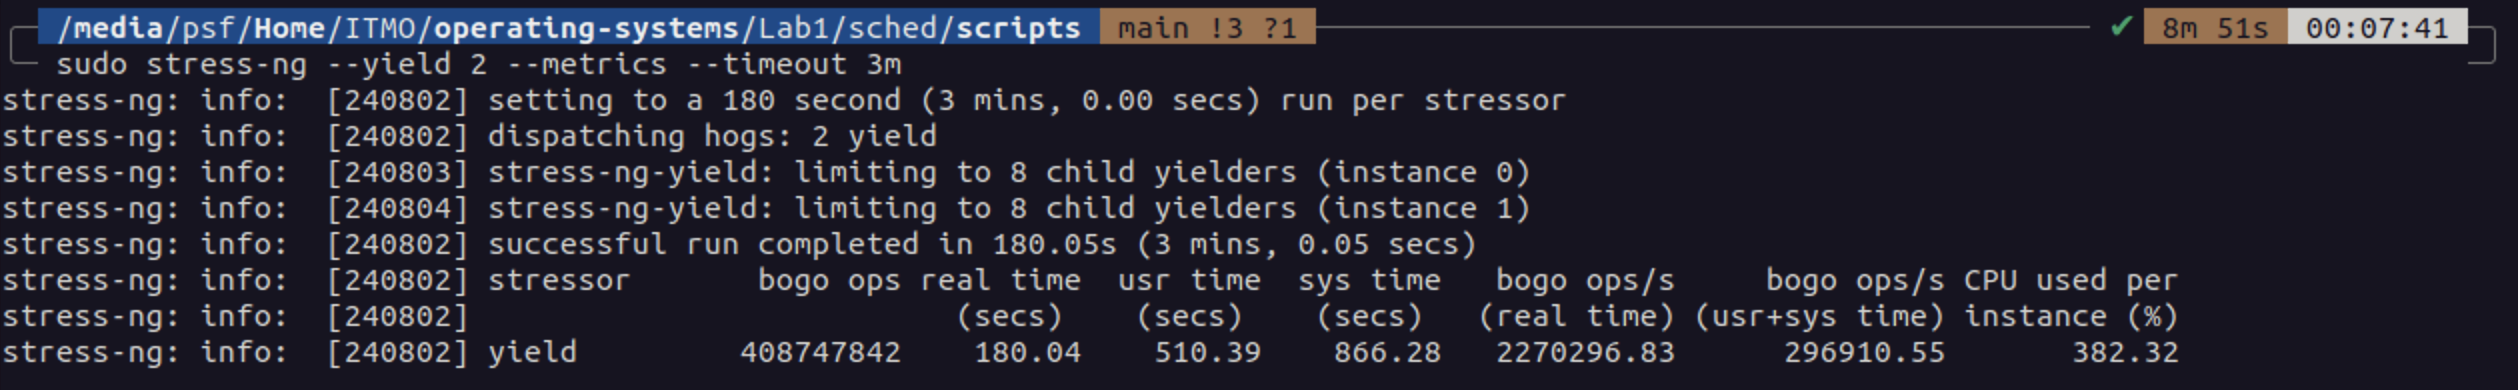
\includegraphics[width=\textwidth]{./sched/image/yield.png}
Запустим \textit{pidstat} с параметрос \textit{-w}:
\nquote{cswch/s}{Total number of voluntary context switches the task made per second.  A voluntary context  switch  occurs
when a task blocks because it requires a resource that is unavailable.}
\nquote{nvcswch/s}{Total  number  of  non voluntary context switches the task made per second.  A involuntary context switch
takes place when a task executes for the duration of its time slice and then is forced to relinquish  the
processor.}
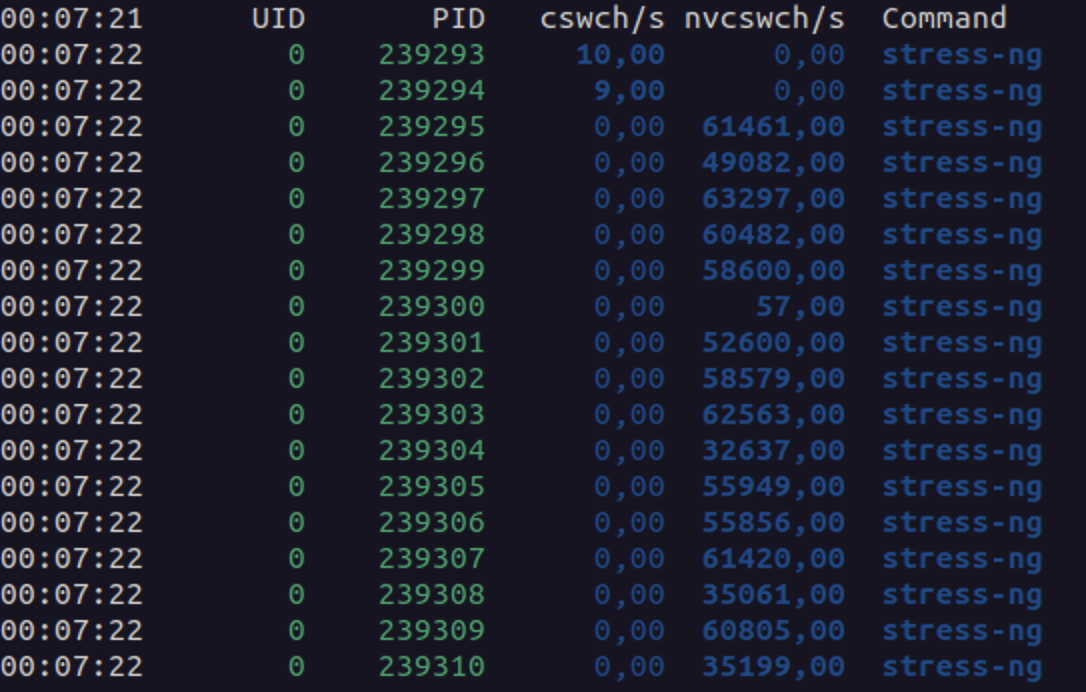
\includegraphics[width=\textwidth]{./sched/image/yield-pidstat.png}
Видим, что исполняются только два процесса, остальные же постоянно меняют контекст.\\
\subsection{schedpolicy}
\nquote{--schedpolicy N}{start  N  workers  that  work  set  the  worker  to  various  available  scheduling policies out of SCHED\_OTHER,
SCHED\_BATCH, SCHED\_IDLE, SCHE\_FIFO, SCHED\_RR and SCHED\_DEADLINE.  For the real time scheduling policies a  random sched priority is selected between the minimum and maximum scheduling priority settings.}
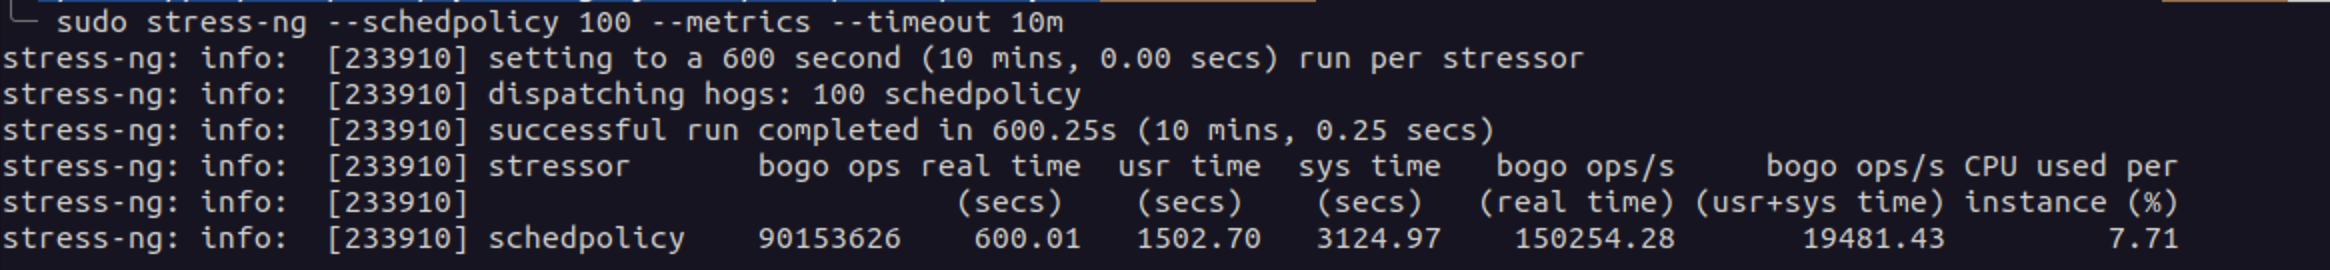
\includegraphics[width=\textwidth]{./sched/image/schedpolicy.png}
С помощью команды \textit{top} мы видим, что политики планирования меняются:\\
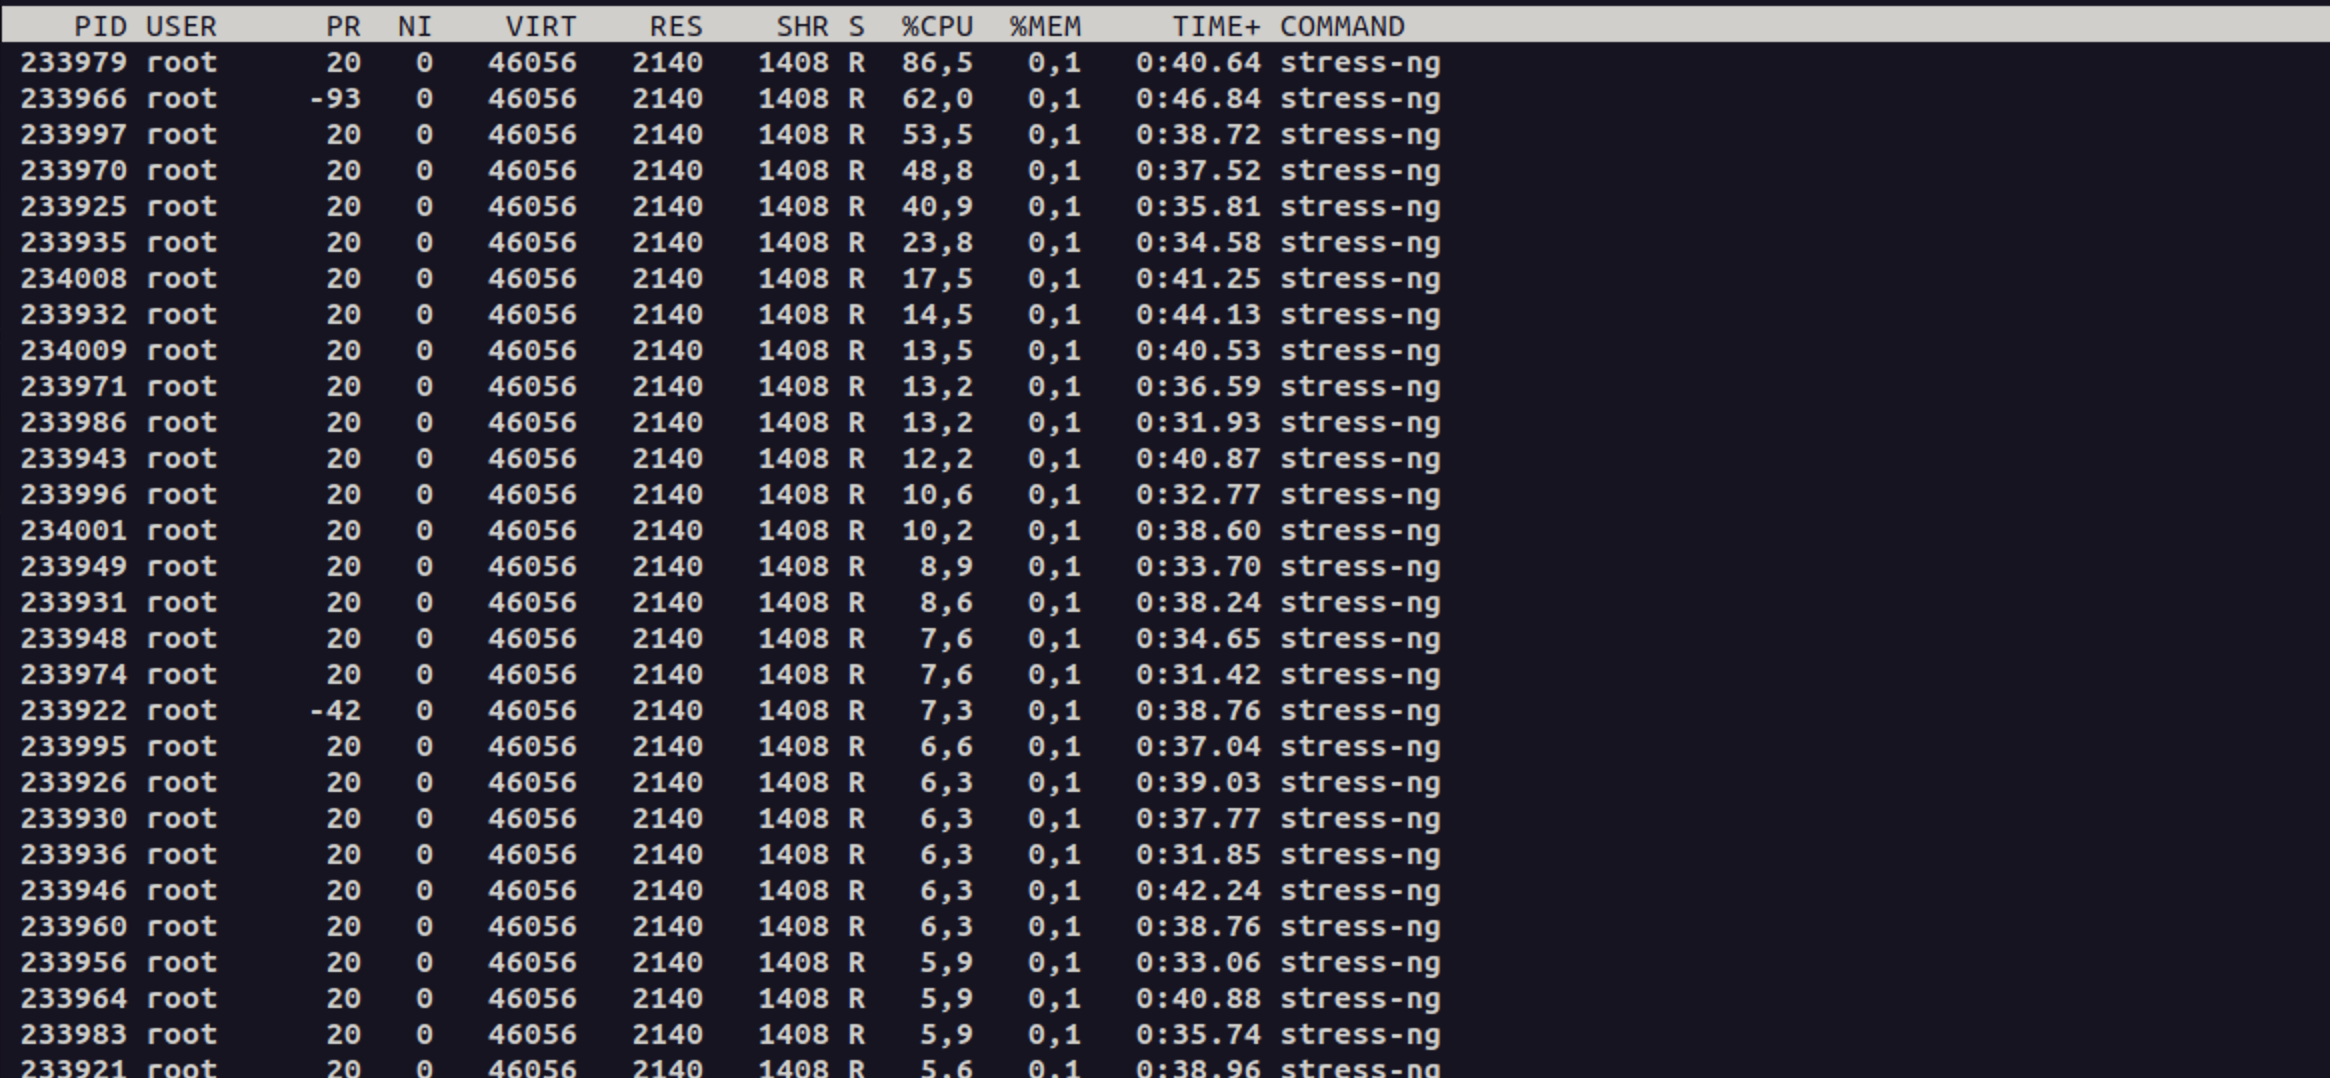
\includegraphics[width=\textwidth]{./sched/image/schedpolicy-top.png}\\
Выберем рандомный процесс и посмотрим как его политики планирования изменяются со временем:
\lstinputlisting[]{sched/scripts/schedpolicy-pidstat.zsh}
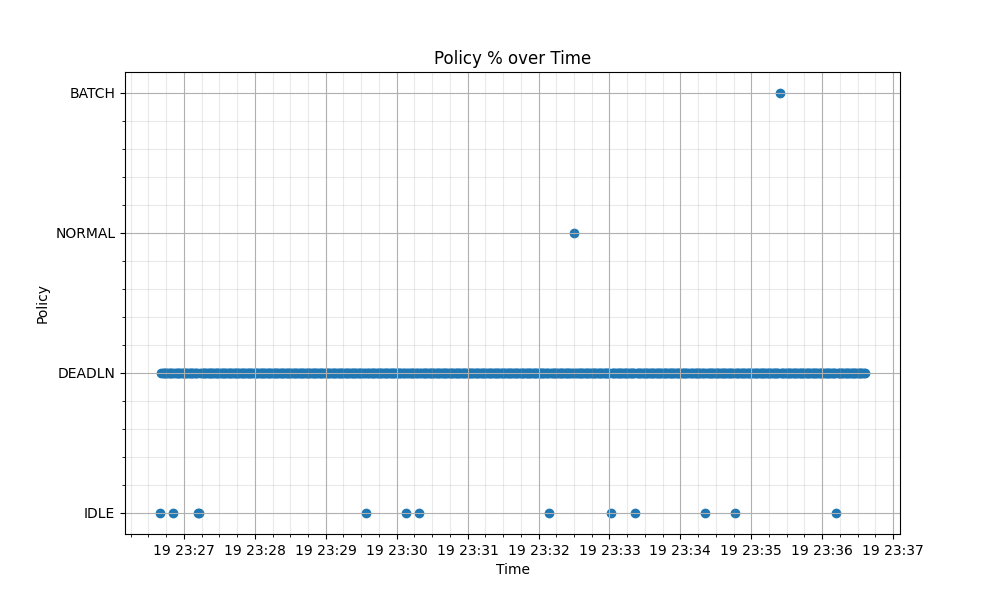
\includegraphics[width=\textwidth]{./sched/image/schedpolicy-pidstat.png}
Видим, что он большую часть работал с политкой DEADLINE, немного с IDLE, и совсем чуть-чуть с NORMAL и BATCH.\\